%%%%%%%%%%%%%%%%%%%%%%%%%%%%%%%%%%%%%%%%%%%%%%
%documentclass és a packegek
%%%%%%%%%%%%%%%%%%%%%%%%%%%%%%%%%%%%%%%%%%%%%%
\documentclass[12pt,a4paper]{article}
\usepackage[utf8]{inputenc}
\usepackage[english]{babel}
\usepackage[T1]{fontenc}
\usepackage{amsmath}
%\usepackage{expl3}
\usepackage{amsfonts}
\usepackage{amssymb}
\usepackage{enumitem}
\usepackage{makeidx}
\usepackage{mathtools}
\usepackage{color}
\usepackage[dvipsnames,tabular]{xcolor}
%\usepackage{tcolorbox}
\usepackage{colortbl}
\usepackage{graphicx}
\usepackage{commath}
\usepackage{lmodern}
\usepackage{fancyhdr}


\usepackage{subfig}
%\usepackage{fancybox}
\usepackage[thinlines]{easytable}
%\usepackage[margin=0.5in]{geometry}
\usepackage[normalem]{ulem}
%\usepackage{blindtext}
\usepackage{float}
\usepackage{fixmath}
\usepackage[colorlinks=false]{hyperref}
\usepackage{indentfirst}
\usepackage{parskip}
\setlength{\parskip}{10 pt}
\setlength{\parindent}{10 pt}
\usepackage{multirow}
\usepackage{gensymb}
\usepackage[titletoc,title]{appendix}
\usepackage{listings}

\usepackage{tikz}
\newcommand*\circled[1]{\tikz[baseline=(char.base)]{
            \node[shape=circle,draw,inner sep=2pt] (char) {#1};}}


\DeclareMathOperator\arctanh{arctanh}
%%%%%%%%%%%%%%%%%%%%%%%%%%%%%%%%%%%%%%%%%%%%%%
%labelek
%%%%%%%%%%%%%%%%%%%%%%%%%%%%%%%%%%%%%%%%%%%%%%

%%%%%%%%%%%%%%%%%%%%%%%%%%%%%%%%%%%%%%%%%%%%%%
%wavy line fekete
%%%%%%%%%%%%%%%%%%%%%%%%%%%%%%%%%%%%%%%%%%%%%%
%\makeatletter
%\def\squiggly{\bgroup \markoverwith{\textcolor{black}{\lower3.5\p@\hbox{\sixly \char58}}}\ULon}
%\makeatother

\newcommand{\be}{\begin{equation}}
\newcommand{\ee}{\end{equation}}
\newcommand{\ket}[1]{{ |#1 \rangle}}
\newcommand{\bket}[1]{{\big|#1\big\rangle}}
\newcommand{\bbra}[1]{{\big\langle#1\big|}}
\newcommand{\bra}[1]{{\langle#1|}}

\DeclareMathOperator{\sign}{sgn}

%%%%%%%%%%%%%%%%%%%%%%%%%%%%%%%%%%%%%%%%%%%%%%
%Margók
%%%%%%%%%%%%%%%%%%%%%%%%%%%%%%%%%%%%%%%%%%%%%%
%\setlength{\topmargin}{-0.3in}
%\setlength{\textheight}{10,0in}
%\setlength{\leftmargin}{0cm}
%\setlength{\oddsidemargin}{-0.2cm}
\setlength{\textwidth}{5.4in}
\def\svgwidth{1.2\textwidth}


%%%%%%%%%%%%%%%%%%%%%%%%%%%%%%%%%%%%%%%%%%%%%%
%Pagestyle
%%%%%%%%%%%%%%%%%%%%%%%%%%%%%%%%%%%%%%%%%%%%%%
%\pagestyle{empty}
\fancyhf{}
\rhead{}
\chead{}
\lhead{}
\cfoot{ \thepage }

%%%%%%%%%%%%%%%%%%%%%%%%%%%%%%%%%%%%%%%%%%%%%%
%Saját színek
%%%%%%%%%%%%%%%%%%%%%%%%%%%%%%%%%%%%%%%%%%%%%%
\definecolor{name}{RGB}{80,160,0}
	{\color{name}}

%%%%%%%%%%%%%%%%%%%%%%%%%%%%%%%%%%%%%%%%%%%%%%
%Newcommands
%%%%%%%%%%%%%%%%%%%%%%%%%%%%%%%%%%%%%%%%%%%%%%
\newcommand{\highlight}[1]{%
\colorbox{name!40}{$\displaystyle#1$}}
%\addto{\captionsenglish}{\renewcommand{\abstractname}{Absztrakt}}
%\addto{\captionsenglish}{\renewcommand{\refname}{Bibliography}}
%%%%%%%%%%%%%%%%%%%%%%%%%%%%%%%%%%%%%%%%%%%%%%
%a colorobox saját verziói
%%%%%%%%%%%%%%%%%%%%%%%%%%%%%%%%%%%%%%%%%%%%%%


%\DeclareMathSizes{10}{10}{7}{10}
\numberwithin{equation}{section}
\begin{document}
\begin{center}
{\Large{Domcsi Jegyzet}}\\
Theoretical modeling of the collective\\ tunneling of a Wigner necklace\\
\today
\end{center}
\pagestyle{empty}
\tableofcontents
\newpage

\setcounter{page}{1}
\pagestyle{plain}
\section{Path integral}

Szöveget kell ide rakni

\begin{equation}
\hat{H} = \frac{\hat{p}^2}{2m} + V(\hat{x})
\end{equation}

\begin{equation}
\int dx\, \ket{x}\bra{x} = \mathbb{I}
\end{equation}

\begin{equation}
\int \frac{dp}{2\pi} \ket{p}\bra{p} = \mathbb{I}
\end{equation}

\begin{equation}
\ket{\Psi} \rightarrow \Psi(x) = \bra{x}\Psi\rangle
\end{equation}

Let's denote $\left.\Psi(x)\right|_{t = t_0} $ by $\Psi_0 (x)$

\begin{equation}
\bra{x} \underbrace{e^{-it\hat{H}} \ket{\Psi_0}}_{\Psi(t)} = \Psi(x,t)
\end{equation}

\begin{align}
\ket{\Psi_0} &= \int dx\, \ket{x}\bra{x}\Psi_0 \rangle \\
&= \int dx\, \Psi_0 (x) \ket{x}\\
\end{align}

\begin{align}
\Psi(x,t) = \int dx' \underbrace{\bra{x} e^{-it\hat{H}}\ket{x'}}_{K(x,x',t)} \underbrace{\bra{x'}\Psi_0 \rangle}_{\Psi_0 (x')}
\end{align}

Making our time variable discretised:
\begin{equation}
t \Rightarrow \Delta t = \frac{t}{N}
\end{equation}

Propagator - The matrix element of the time evolution(t.e.) operator using the previous discretised time, between (now) some arbitrary initial and final position, This is denoted in Feynman's book by $K(x,x^\prime,t)$  or in Altland \& Simons's book by $G(a,\pm a,\tau)$ in the case of instantons:
\begin{equation} \label{eq1:11}
\bra{x}e^{-i\Delta t H} \cdot e^{-i\Delta t H} \cdots e^{-i\Delta t H}\ket{x'} 
\end{equation}

The t.e. operator can be decomposed in the following way:
\begin{equation}
e^{-i\Delta t H} = e^{-i \Delta t \frac{p^2}{2m}}\, e^{-i \Delta t V(x)} + \mathcal{O} (\Delta t^2)
\end{equation}

The series of $e^{-iax}$ at $x = 0$:
\begin{equation}
e^{-i a x} \approx 1 + (-i a )\, x - \frac{1}{2}x^2 (-i a)^2 + \dots
\end{equation}

and of $e^{-i a x}\, e^{-i b x}$ at $x = 0$:
\begin{equation}
e^{-i a x}\, e^{-i b x} \approx 1 + (-i)(a+b)\, x - \frac{1}{2}(a^2 + b^2 + \left\lbrace a,b \right\rbrace) + \dots
\end{equation}

The decomposition of the time evolution op. can be done in another, so called Trotter decomp. way:
\begin{equation}
e^{-iH \Delta t} = e^{-i \frac{\Delta t}{2} T}\, e^{-i\Delta t V} \, e^{-i \frac{\Delta t}{2} T}
\end{equation}
This approximation is a better one compared to just separating T and V from the hamiltonian $\rightarrow$ $\mathcal{O}(\Delta t^3)$\\
Let's now calculate the first term using the simpler '$T + V$' decomposition. 
\begin{align}
\int \dots \int {\rm{d}}x_{N-1} \dots {\rm{d}} x_1 &\bra{x} e^{- \frac{i}{\hbar} H \Delta t} \ket{x_{N-1}}\, \bra{x_{N-1}} e^{- \frac{i}{\hbar} H \Delta t} \ket{x_{N-2}} \dots \\
\cdot &\bra{x_1} e^{- \frac{i}{\hbar} H \Delta t} \ket{x_{0}}  \nonumber
\end{align} 

Here we can substitute in the unity, writing here only the last terms:
\begin{equation}
\dots e^{-i V \Delta t}   \int {\rm{d}}x_1 \ket{x_1} {\bra{x_1}\int \frac{{\rm{d}}p_1}{2\pi} \ket{p_1}\bra{p_1}\,e^{-i T \Delta t}\, e^{-i V \Delta t} \ket{x_0}}
\end{equation}

%\begin{equation}
%{\bra{x_1}\, e^{-i V \Delta t} \ket{x_0}} = \bra{x_1}x_0\rangle\, e^{-i V(X_0) %\Delta t}
%\end{equation}
%Similarly

%\begin{equation}
%\bra{p_1} e^{-i T \Delta t}\ket{x_1} = e^{-i \frac{p_1 ^2}{2m} \Delta t} %\underbrace{\bra{p_1}x_1\rangle}_{e^{-i p_1 x_1 / \hbar} \frac{1}{\sqrt{2 \pi \hbar}}}
%\end{equation}



\begin{align}
&\int \frac{dp_1}{2\pi} \ket{p_1}\bra{p_1} \, e^{-i\Delta t T_1}\, e^{-i\Delta t V} \ket{x_0} \\
= &\int \frac{dp_1}{2\pi} \ket{p_1} e^{-i \frac{p_1^2}{2m} \Delta t }\bra{p_1}x_0\rangle e^{-i\Delta t V} \\
= &\int \frac{dp_1}{2\pi} \ket{p_1} e^{-i \frac{p_1^2}{2m} \Delta t } e^{-i p_1 x_0}e^{-i\Delta t V} \\
= &\mathcal{I}
\end{align}

The next term then comes as:
\begin{align} \label{eq1:22}
&\int dx_1 \ket{x_1}\bra{x_1} e^{-i\Delta t V} \cdot \mathcal{I} \\
= &\int {\rm{d}}x_1 \ket{x_1} e^{-i V(x_1 ) \Delta t} \int \frac{{\rm{d}}p_1}{2\pi} \bra{x_1} p_1 \rangle e^{-i \frac{p_1^2}{2m} \Delta t} \, e^{-i p_1 x_0} e^{-i V(x_0) \Delta t}\\
= &\int {\rm{d}}x_1 \ket{x_1} e^{-i V(x_1 ) \Delta t} \int \frac{{\rm{d}}p_1}{2\pi} e^{-i \frac{p_1^2}{2m} \Delta t} e^{i (x_1 - x_0) p_1} e^{-i V(x_0) \Delta t}
\end{align}

Dealing with the exponents containing $p_1$:
\begin{align}
\exp\left\lbrace \frac{-i\Delta t }{2m}p_1^2 + i(x_1 - x_0) p_1 \right\rbrace
\end{align}

\begin{align} \label{eq1:27}
\left\lbrace \dots \right\rbrace &= \frac{-i\Delta t }{2m}p_1^2 + i(x_1 - x_0) p_1 \\
&= \frac{-i\Delta t }{2m} \left( p_1 - \frac{x_1 - x_0}{\Delta t} m \right)^2 + i\frac{m}{2} \Delta t \left( \frac{x_1 - x_0}{\Delta t}\right)^2 \\
\end{align}

Integrating over eq.(\ref{eq1:27}) by $p_1$ as a gaussian integral:
\begin{align}
I^\prime &= \int \frac{{\rm{d}} p_1 }{2\pi} \exp\left\lbrace \frac{-i\Delta t }{2m} \left( p_1 - \frac{x_1 - x_0}{\Delta t} m \right)^2 + i\frac{m}{2} \Delta t \left( \frac{x_1 - x_0}{\Delta t}\right)^2 \right\rbrace \\
&= \sqrt{\frac{m}{2 \pi i \Delta t(\hbar)}}\\
&= N_{\Delta t} \\
\end{align}

eq.(\ref{eq1:22}) then will become:
\begin{equation}
\int dx_1 \ket{x_1} e^{-i \Delta t (V(x_1) + V(x_0))}\, e^{i\frac{m}{2} \Delta t \left( \frac{x_1 - x_0}{\Delta t}\right)^2} N_{\Delta t}
\end{equation}

if we follow this trhough in eq.(\ref{eq1:11}) we would end up:
\begin{equation}
N_{\Delta t}^N \int {\rm{d}}x_1 \dots {\rm{d}}x_{N-1} \exp\left\lbrace i \left( {\Delta t \sum\limits_{i=1}^N \frac{m}{2} \left( \frac{x_i - x_{i-1}}{\Delta t} \right)^2} - \Delta t \sum\limits_{i=0}^{N-1} V(x_i)\right) \right\rbrace
\end{equation}

\begin{align*}
t_i &= t_0 + i\cdot \Delta t \\
x_i &= x(t_i)
\end{align*}

The squared term in the first sum looks like a numerical derivative. The first sum can be rewritten as an Integral:

\begin{equation}
1 \Rightarrow \int\limits_{t_0}^{t} {\rm{d}} t^\prime \frac{m}{2} \left( \frac{dx}{dt^\prime} \right)^2
\end{equation}

Similarly for the second sum:

\begin{equation}
2 \Rightarrow \int\limits_{t_0}^{t}\, {\rm{d}} t^\prime V(x(t^\prime))
\end{equation}

\begin{equation}
K(x,x^\prime,t) = \underbrace{\lim_{\Delta t \rightarrow 0} N_{\Delta t}^N \int {\rm{d}}x_1 \dots {\rm{d}} x_{N-1}}_{\int \mathcal{D}x} \exp \underbrace{ \left\lbrace i \int\limits_{t_0}^t {\rm{d}}t^\prime \mathcal{L}(x,\dot{x},t)\right\rbrace}_{S(x^\prime,x,t,t^\prime)} 
\end{equation}

Useful notation for the future:
\begin{equation}\label{1:39}
\mathcal{D}x := \lim_{\epsilon\text{ or } \Delta t \rightarrow 0} \left( \frac{m}{2 \pi i \hbar \Delta t}\right)^{1/2} \prod\limits_{n=1}^{N-1} \left( \frac{m}{2 \pi i \hbar \Delta t}\right)^{1/2} dx_n
\end{equation}


\begin{equation}
K(x,x^\prime,t) = \int\limits_{x^\prime (t_0)}^{x(t)} \mathcal{D}x \,\, e^{i\frac{1}{\hbar} \int {\rm{d}}t \mathcal{L}(x,\dot{x})}
\end{equation}





\subsection{Gaussian integrals}
%Altland,Simons 102-

\subsubsection{one dimensional case}
If Re($a$)>0
\begin{equation}
\int\limits_\infty^\infty \text{dx } e^{-\frac{a}{2} x^2} dx= \frac{2 \pi}{a}
\end{equation}

\begin{equation}
\int\limits_\infty^\infty \text{dx } e^{-\frac{a}{2} x^2} x^2 = \sqrt{\frac{2 \pi}{a^3}}
\end{equation}

If the exponent is not purely quadratic:
\begin{equation}
\int\limits_\infty^\infty \text{dx } e^{-\frac{a}{2}x^2 + bx} = \frac{2\pi}{a} e^{\frac{b^2}{2a}}
\end{equation}

This can be performed by changing the variable from $x \rightarrow y = x + \frac{b}{a}$.

For complex arguments, if $Re(\omega) >0$ and $\tilde{z}$ represents the complex conjugate of $z$:
\begin{equation}
\int d(z,\tilde{z}) e^{-\tilde{z}\omega z} = \frac{\pi}{\omega}
\end{equation}

\subsubsection{more than one dimensional cases:}
First, the real case:
\begin{equation}
\int \,d\vec{v}\, e^{-\frac{1}{2}\vec{v}^T \textbf{A} \vec{v}} = (2\pi)^{N/2} \det\textbf{A}^{-1/2}
\end{equation}

\begin{equation}
\int d\vec{v}\, e^{-\frac{1}{2}\vec{v}^T \textbf{A}\vec{v} +\vec{j}^T \vec{v}} = (2\pi)^{N/2} \det A^{-1/2} e^{\frac{1}{2} \vec{j}^T \textbf{A}^{-1}\vec{j}}
\end{equation}
Here $\vec{j}$ is an arbitrary N component vector, \textbf{A} is an NxN symmetric positive definite matrix.

Complex case:
\begin{equation}
\int d(\vec{v}^\dagger,\vec{v}) e^{-\vec{v}^\dagger \textbf{A}\vec{v}} = \pi^N \det \textbf{A}^{-1}
\end{equation}


\subsection{Free particle}

Lagrangian of the free particle:
\begin{equation}
\hat{H} = \frac{\hat{p}^2}{2m} \,\rightarrow\, \mathcal{L} = \frac{1}{2}m\dot{x}^2
\end{equation}

First the propagator for 1 dimension:
\begin{align}
K(x,\dot{x},t) &= \bra{x_b , t_b} x_a, t_a \rangle \\
&= \bra{x_b} e^{-iH(t_b-t_a)/\hbar} \ket{x_a} \\
&= \int dp \bra{x_b}p\rangle \bra{p}e^{-i (p^2/2m)t/\hbar} \ket{x_a} \\
&=\int dp \frac{1}{\sqrt{2\pi \hbar}} e^{i p x_b /\hbar} \bra{p}e^{-i (p^2/2m)t/\hbar} \ket{x_a} \\
&= \int dp \frac{1}{{2\pi \hbar}} e^{-i \frac{t}{2m\hbar} (p - mx/t)^2 + i \frac{mx^2}{2\hbar t}}\\
&= \frac{1}{{2\pi \hbar}} \sqrt{\frac{2 \pi m \hbar}{i t}} e^{\frac{i mx^2}{2 \hbar t}}\\
&= \sqrt{\frac{m}{2 \pi i \hbar t}}  e^{\frac{i m x^2}{2 \hbar t}}\\
&= \sqrt{\frac{m}{2 \pi i \hbar (t_b-t_a)}}  e^{\frac{i m (x_b-x_a)^2}{2 \hbar (t_b-t_a)}}
\end{align}

In Feynman's book $t_b - t_a$ is denoted by the timescale division $\epsilon$.

\begin{equation}
K_{\text{free}} = \lim_{\epsilon \rightarrow 0} \left( \frac{m}{2\pi i \hbar \epsilon}\right)^{N/2} \int \dots \int \exp\left\lbrace \frac{i m }{2\hbar \epsilon}\sum\limits_{i = 1}^N (x_i - x_{i-1})^2  \right\rbrace dx_1 \dots dx_{N-1}
\end{equation}
Here taking only the first integration variable $dx_1$ a gaussian integral has to be evaluated and then multiplied by the next exponent and norm factor pair to calculate a very similar gaussian. In the end we get back the same result.

\subsection{Quantum particle in a well - Harmonic oscillator}
Lets now consider a symmetric potential ($V(q) = V(-q)$; $V(0) = 0$) well in one dimension:

\begin{equation}
K(0,0;t) = \int\limits_{q(0) = q(t) = 0} \mathcal{D}q\,\, e^{\frac{i}{\hbar}\int_0^t dt' \mathcal{L}(q,\dot{q})}
\end{equation}

In order to solve this we must know the result of the Euler-Lagrange equation for the classical motion with the above boundary conditions. One solution to this is $q_{cl}(t) =0$

One can expand the path within the action around a fixed classical path:
\begin{equation}
r(t) = q (t) - q_{cl}(t)
\end{equation}

the boundary conditions regarding this $r(t)$ is the following:
\begin{equation}
r(0) = r(t) = 0
\end{equation}

where the deviation from the classical path is:

\begin{equation}
q (t) = \sum\limits_{n = 0}^{\infty} c_n \tilde{x}_n(t)
\end{equation}

we expect $q_{cl}$ to fulfil the boundary conditions as in the case of $eta$ such that it's vanishes at $0$ and $t$. The consequence of this is that we can rewrite eq.(\ref{1:39}) as follows
\begin{equation}
\mathcal{D}[x] = \mathcal{D}[r] = \prod_n \frac{dc_n}{\sqrt{2\pi\hbar}}
\end{equation}

\paragraph{Saddle point approximation} 
The action can be written
\begin{align}
S[q] &= S[q_{cl}] + \frac{1}{2}  \int dt \int dt' r(t) \left.\frac{\delta^2 S[q]}{\delta q(t) \delta q(t')} \right|_{q = q_{cl}} r(t') + \mathcal{O}(r^3) \\
&= S[q_{cl}] + \frac{1}{2} \int\limits_{0}^{t} dt\, r(t)\, \hat{F}(q_{cl})\, r(t)\\
&= S[q_{cl}] + \frac{1}{2} \int dt\, r(t)\, \left[ m\partial^2_t + V^{''}(q_{cl}(t))  \right]\, r(t)
\end{align}

\begin{equation}
\hat{F}(q_{cl}) = \left[ -m \frac{d^2}{dt^2} + \frac{d^2 V(q_{cl})}{dx^2}  \right]
\end{equation}

The eigeneq. of this operator

\begin{equation}
\hat{F}(q_{cl}) \tilde{x}_n (t) = \lambda_n \tilde{x}_n (t)
\end{equation}

\begin{equation}
S[q] = S[q_{cl}] + \frac{1}{2}\sum_n \lambda_n c_n^2 + \mathcal{O}(r^3)
\end{equation}

Substitute back these into the propagator:

\begin{align}\label{dc0}
K(q_i,q_f;t) &= \mathcal{N} \int \mathcal{D}q\, e^{-\frac{i}{\hbar} S[q]}\\
&\simeq \mathcal{N} e^{-\frac{i}{\hbar} S[q_{cl}]} \int \mathcal{D}r e^{-\frac{i}{2\hbar} \int\limits_{0}^t dt r(t) \hat{F}(q_{cl}) r(t)} \\
&= \mathcal{N} e^{-\frac{i}{\hbar} S[q_{cl}]} \prod_n \int \frac{dc_n}{\sqrt{2\pi \hbar}} e^{-\frac{i}{2\hbar} \sum_n \lambda_n c^2_n} \\
&= \mathcal{N} e^{-i S[q_{cl}]/\hbar} \prod_n \lambda_n^{-1/2} \\
&= \mathcal{N} e^{-i S[q_{cl}]/\hbar} \left(\det \hat{F}[q_{cl}]\right)^{-1/2}
\end{align}

Get back to the single well potential, the second derivative of the potential if V  is
$$
V = \frac{1}{2}m \omega^2 x^2 \quad \rightarrow \quad V^{''}(q) = m\omega^2
$$

So the propagator can be written as:
\begin{equation}
K(0,0;t) \simeq \mathcal{N} \det\left( -m(\partial_t^2 + \omega^2)/2  \right)^{-1/2}
\end{equation}

for the eigenvalues we have to solve the following:
\begin{equation}
-\frac{m}{2} (\partial^2_t + \omega^2) r_n = \lambda_n r_n
\end{equation}

Here $r(t')$ can be given in a general way:
\begin{equation}
r_n(t') = a_n \sin\left(\frac{n \pi t^{'}}{t}\right) + b_n \cos\left(\frac{n\pi t^{'}}{t}\right)
\end{equation}

but the boundary conditions has to be fulfilled, and the normalization is taking care of $a_n$'s factor.
\begin{equation}
r_n(t') = \sin\left(\frac{n \pi t^{'}}{t}\right) \,\rightarrow\, \lambda_n = m[(n\pi/t)^2 - \omega^2]/2
\end{equation}

The determinant then becomes
\begin{equation}
\det (-m(\partial_t^2 + \omega^2)/2)^{-1/2} =   \prod_{n=1}^\infty \left[ \frac{m}{2}\left(\left( \frac{n \pi}{t}  \right)^2 - \omega^2\right) \right]^{-1/2}
\end{equation}

Here comes the magic, here we have to massage some sense out of this infinity product, and work out the normalization factor on the front. It it seems if we set $\omega$ to zero, then it renders the potential absent for this case, but then it becomes the free particle, where the same $\mathcal{N}$ factor emerges. By this logic this last expression can be regularized with the free particle propagator:
\begin{equation}
K(0,0;t) = \frac{K(0,0;t)}{K_{free}(0,0;t)}K_{free}(0,0;t)
\end{equation}

\begin{align}
K(0,0;t) &= \frac{\mathcal{N} \prod_{n=1}^\infty \left[ \frac{m}{2}\left(\left( \frac{n \pi}{t}  \right)^2 - \omega^2\right) \right]^{-1/2}}{\mathcal{N} \prod_{n=1}^\infty \left[ \frac{m}{2}\left( \frac{n \pi}{t}  \right)^2  \right]^{-1/2}} \sqrt{\frac{m}{2 \pi i \hbar t}} \\
&= \prod_{n=1}^\infty \left[1- \left(\frac{\omega t}{n\pi}\right)^2  \right]^{-1/2} \sqrt{\frac{m}{2 \pi i \hbar t}} \\
&= \sqrt{\frac{\omega t}{\sin(\omega t)}} \sqrt{\frac{m}{2 \pi i \hbar t}}\\
&= \sqrt{\frac{m\omega}{2\pi i \hbar \sin(\omega t)}}
\end{align}

\newpage
\section{Instanton}
If we now consider a double well potential, where the particle's energy is much lower than the presented potential barrier, then the transfer between the 2 potential minima is by tunneling. There's no calssical path connecting the minima. To resolve this we can consider the time argument present in the path integral as a generally complex quantity.

\paragraph{Wick rotation} The matrix element with the $t = -i\tau$ time parameter change :

\begin{equation}
K_E (a,\pm a; \tau) = \bra{a} \exp\left( -\frac{\tau}{\hbar} H \right) \ket{\pm a}
\end{equation}
The real time amplitudes can be obtained by $\tau \rightarrow it$.

\begin{equation}
iS = i\int dt \left( \frac{m}{2}\dot{x}^2 - V[x]  \right) \rightarrow i (-i)\int d\tau \left( -\frac{m}{2}\dot{x}^2 - V[x]  \right) = -\int d\tau \mathcal{L}[x] = -S_E
\end{equation}

Thus this Wick rotation makes the potential upside down. In the inverted potential picture one could obtain a classical path that connects the two potential minima:
\begin{itemize}
\item the particle stays at rest at $\pm a$ from 0 to $\tau$
\item the particle goes from $\pm a$ to $\mp a$
\end{itemize}

The first case would give us the zero point motion of the particle, which gives back the harmonic oscillator calculated above.

The particles going from $a$ to $-a$ are called instantons, and anit-instantons if we change signs of the final and inital points.

at $\tau = - \infty$ $v(-\infty) = 0$ where $x=\pm a$ thus the energy of the single particle is 0.
\begin{equation}
\frac{m\dot{x}^2}{2} - V[x] = 0
\end{equation}

\begin{equation}
\dot{x} = \sqrt{\frac{2V[x]}{m}}
\end{equation}

the action of the instanton then can be calculated:
\begin{equation}
S_E = \int\limits_{-\infty}^\infty \, m \dot{x}^2\,d\tau = \int \limits_{-a}^a \sqrt{\frac{2V[x]}{m}}\,m\, dx = \int \limits_{-a}^a \sqrt{{2mV[x]}}\, dx
\end{equation}

\subsection{The instanton solution}

Now we want to calc. the calssical path for a particle in the upside down potential:
Let's say that the potential is in the form of 
\begin{equation}
V(x) = -\frac{\alpha}{2}x^2 + \frac{\beta}{4}x^4
\end{equation}

\begin{equation}
\frac{\partial V}{\partial x} = -\alpha x + \beta x^3 = 0 \rightarrow \beta x^3 = \alpha
\end{equation}

Here we could make the variable change:
\begin{equation}
\chi = \frac{x}{x_0}
\end{equation}
 where $x_0$ is from the previous derivation:
 \begin{equation}
 x_0 = \pm \sqrt{\frac{\alpha}{\beta}}
 \end{equation}

The potential's form then can be rewritten:
\begin{equation}
V(\chi) = -\frac{\alpha}{2}\chi^2 \frac{\alpha}{\beta} + \frac{\beta}{4}\chi^4 \left( \frac{\alpha}{\beta}\right)^2
\end{equation}

\begin{equation}
S = \int\limits_{-\infty}^\infty d\tau \left\lbrace \frac{m}{2} x_0^2 \dot{\chi}^2 + \frac{\alpha^2}{2\beta} \left( \frac{1}{2} \chi^4 - \chi^2  \right) \right\rbrace
\end{equation}

Introducing a new cplx time variable:
\begin{equation}
\tau = \tau_0 y
\end{equation}

\begin{equation}
\frac{mx_0^2}{2} \left( \frac{d\chi}{d\tau}\right)^2 \Rightarrow \frac{mx_0^2}{\tau_0^2} = \frac{\alpha^2}{2\beta} = x_0^2 \alpha \Rightarrow \tau_0 = \sqrt{\frac{m}{\alpha}}
\end{equation}

\begin{equation}
S = x_0^2 \alpha \tau_0 \int\limits_{-\infty}^\infty dy \left\lbrace \frac{1}{2} \left( \frac{d\chi}{dy}\right)^2 - \frac{1}{2}\chi^2 + \frac{1}{4}\chi^4 \right\rbrace
\end{equation}

We can shift this, so the minima of the inverted potential lies at 0:

If we consider the next section's nondimensionalization then we could end up with the following
\begin{align}
V(x) \rightarrow V(x) - V(x_0) &=\\
&= -\frac{\alpha}{2}x^2 + \frac{\beta}{4}x^4 + \frac{\alpha}{2}x_0^2 - \frac{\beta}{4}x_0^4\\
&= \frac{\alpha^2}{\beta}\frac{1}{4} \left( \chi^2 - 1 \right)^2
\end{align}

\begin{equation}
S = S_0 \int_{\infty}^\infty dy\left\lbrace \frac{1}{2}\left( \frac{d\chi}{dy}\right)^2 + v(\chi)\right\rbrace
\end{equation}


As stated before the energy of the particle at times $\pm \infty$ is 0:
\begin{equation}
\frac{1}{2}\dot{\chi}^2 - v(\chi) = \varepsilon
\end{equation}


\begin{align}
\frac{1}{2}\dot{\chi}^2 &= v(\chi) \\
\dot{\chi} &= \sqrt{2} \frac{1}{2} (\chi^2 -1 )\\
y &= \int d\chi \frac{1}{(1-\chi^2)}\sqrt{2} = \sqrt{2} \arctanh(\chi)
\end{align}

\begin{equation}\label{clpath}
\chi(y) = \tanh(y/\sqrt{2}) \, \Rightarrow \, x(\tau) = \sqrt{\frac{\alpha}{\beta}} \tanh(\tau/\sqrt{2}\tau_0)
\end{equation}

\paragraph{Tunneling calc.}
\begin{align}
S/S_0 &= \int\limits_{-\infty}^\infty dy 2 \frac{1}{2} \left(  \frac{d\chi}{dy} \right)^2  \\
&= \int dy \left( \frac{d}{dy} \tanh(y/\sqrt{2} \right)^2\\
&= \int dy \left(\frac{1}{\sqrt{2}} \frac{1}{\cosh^2(y/sqrt{2}}) \right)^2 \\
&= \int dy \frac{1}{2} \frac{1}{\cosh^4 (y/\sqrt{2}} \\
&= \frac{2 \sqrt{2}}{3}
\end{align}


We can now reparametrize the time:
\begin{equation}
z = \tanh(y/r) 
\end{equation}


\begin{align}
\frac{d\chi}{dy} &= \frac{d\chi}{dz} \frac{dz}{dy} \\
&= \frac{d\chi}{dz} \frac{1}{r} \frac{1}{\cosh^2(y/r)}\\
&= \frac{1}{r} (1-z^2) \frac{d\chi}{dz}
\end{align}
Substituting the new time parameter back to our action integral
\begin{equation}
S = S_0 \int\limits_{-1}^1 dz \left\lbrace \frac{1-z^2}{2r} \left( \frac{d\chi}{dz}\right)^2 + \frac{r}{1-z^2} v(\chi) \right\rbrace
\end{equation}

\newpage
\subsection{Action integral calculation for 1 particle Instanton tunneling}

The confinement potential is in the form of:
\begin{equation}
{V}(x) = \frac{\alpha}{2} x^2 + \frac{\beta}{4} x^4
\end{equation}

One could shift the potential in a way that in the (one particle) equlibrium, the particles potential energy is zero:
$$
\tilde{V}(x) \rightarrow V(x) - V(x_0)
$$

\[
\frac{\partial V(x)}{\partial x} = x^3 - a x = 0 \rightarrow x_0 = \pm \sqrt{a}
\]

This way the potential's minima will be at 0:
\begin{align}\label{eq20}
\tilde{V}(x) &= \frac{1}{4} x^4 - \frac{a}{2}x^2 - \left( \frac{1}{4}a^2 - \frac{a}{2}a\right)\\ \nonumber
 &= \frac{1}{4}x^4 - \frac{a}{2}x^2 + \frac{a^2}{4} \\ \nonumber
 &= \frac{1}{4} (x^2 - a)^2
\end{align}

Let's use now the nondimensionalized formalism eq.(\ref{eq16}) with this shifted potential. For 1 particle the action integral takes the form:
\begin{equation}
\frac{S}{\hbar} = S_0 \int\limits_{-\infty}^\infty  dy \left\lbrace \frac{1}{2} \left(\frac{\partial \tilde{\chi}}{\partial y} \right)^2 + v(\tilde{\chi})\right\rbrace
\end{equation}
Where $v(\tilde{\chi}) $ denotes the nondimensionalized form of eq.(\ref{eq20}).


\begin{figure}[H]
\centering
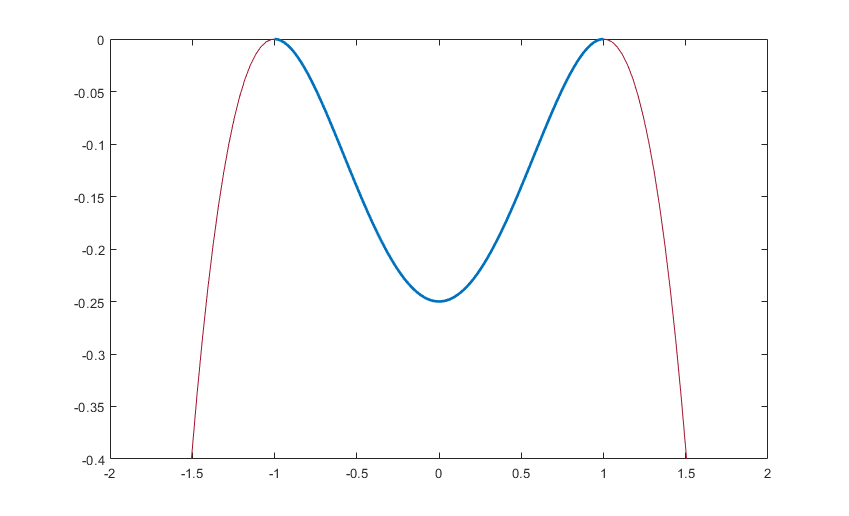
\includegraphics[width = 0.7\textwidth]{inverted_pot}
\caption{Inverted potential}
\end{figure}
To solve this, we can use he E-L equation:
\[
\frac{d}{dy}\frac{\partial L}{\partial \dot{\tilde{\chi}}} = \frac{\partial L}{\partial \tilde{\chi}}
\]

\begin{equation}
\frac{d^2 \tilde{\chi}}{dy^2} = \frac{\partial v(\tilde{\chi})}{\partial \tilde{\chi}}
\end{equation}

The particle's energy in the equilibrium positions is zero, thus
\begin{align}
\nonumber
\frac{1}{2}\left( \frac{d \tilde{\chi}}{d y}\right)^2 &= v(\tilde{\chi}) \\
\frac{d \tilde{\chi}}{d y} &= \sqrt{2} \frac{1}{2} (\tilde{\chi} ^2 -a)
\end{align}

\begin{equation}
y = \int d\tilde{\chi} \frac{1}{(1-\tilde{\chi}^2)}\sqrt{2} = \sqrt{2} \arctanh(\tilde{\chi})
\end{equation}


\begin{equation}
\tilde{\chi}(y) = \tanh(y/ \sqrt{2})
\end{equation}




\subsection{Tunneling calculation}

\begin{align}
S &= S_0 \int\limits_{-\infty}^\infty dy 2\cdot \frac{1}{2} \left( \frac{d \tilde{\chi}}{d y}\right)^2 \nonumber\\
&= S_0 \int dy \left( \frac{d}{dy} \frac{1}{\cosh^2(y/\sqrt{2)}} \right)^2 \nonumber \\
&= S_0 \int dy \frac{1}{\cosh^4 (y/\sqrt{2})}\\
&= S_0 \frac{2 \sqrt{2}}{3} \nonumber
\end{align}

\subsection{Reparametrization of time}

Let $z$ be:
\begin{equation}
z = \tanh(y/r)
\end{equation}

\begin{align}
\frac{d\tilde{\chi}}{dy} &= \frac{d\tilde{\chi}}{dz} \frac{dz}{dy} \nonumber \\
&= \frac{d\tilde{\chi}}{dz} \frac{1}{r}\frac{1}{\cosh^2(y/r)} \nonumber \\
&= \frac{(1-z^2)}{r} \frac{d\tilde{\chi}}{dz}
\end{align}

Substituting this back in the action integral:

\begin{equation}
\frac{S}{\hbar} = \int\limits_{-1}^1 dz \left\lbrace \frac{1-z^2}{2r} \left( \frac{d \tilde{\chi}}{dz} \right)^2 + \frac{r}{1-z^2} v(\tilde{\chi}) \right\rbrace
\end{equation}


\subsection{Instanton fluctuation determinant}

\begin{align}
K(a,-a,\tau) &= \bra{a} e^{-\frac{\tau}{\hbar}H} \ket{-a} \\
&= N \det (-\partial_\tau ^2 + V^{''}(\chi))^{-1/2} e^{\frac{S_E (\chi_{I})}{\hbar}}\\
\end{align}

Now we can normalize this using the results from the harmonic oscillator case:

\begin{equation}
N \det (-\partial_\tau ^2 + V^{''}(\chi))^{-1/2} = N \det (-\partial_\tau ^2 + w^2)^{-1/2} \left\lbrace\frac{ \det (-\partial_\tau ^2 + V^{''}(\chi))}{\omega^{-2}\det (-\partial_\tau ^2 + w^2)}\right\rbrace^{-1/2}
\end{equation}

We know only interested in the ratio between the two determinants. Lets start with the potential:
\begin{align}
V(\chi) &= \frac{1}{4}(\chi^2 -a^2)^2 \\
&= \lambda (\chi^2 - a^2 )^2 \\
V'(\chi) &= \lambda (4\chi^3 - 4a^2 x) \\
V''(\chi) &= \lambda (12\chi^2 - 4a^2)
\end{align}

simplification with:
\begin{equation}
\omega^2 = 8\lambda a^2
\end{equation}

and substituting back $\chi$ into the equations:
\begin{equation}
\chi = \pm a \tanh (\frac{\omega}{2} (\tau - \tau_0))
\end{equation}

\begin{align}
V''(\chi) &= \lambda (12 a^2 \tanh^2 (\omega /2 (\tau - \tau_0)) - 4a^2)\\
&= \frac{\omega^2}{2} (3 \tanh^2 (\omega /2 (\tau - \tau_0)) - 1) \\
&= \frac{\omega^2}{2} \left( 2 - \frac{3}{\cosh^2 (\frac{\omega}{2} (\tau-\tau_0)}\right) \\
&= \omega^2 \left( 1 - \frac{3}{2\cosh^2 (\frac{\omega}{2} (\tau-\tau_0)}\right)
\end{align}

let's set $\tau_0$ to zero and write the determinant:
\begin{equation}
-\frac{\partial^2}{\partial\tau^2} r_n (\tau) + V''(\chi) r_n (\tau) = \varepsilon_n r_n(\tau)
\end{equation}

We need to solve this Schrödinger like equation. (now with simplified notation)

\begin{equation}
\partial^2_\tau r - (\omega^2 - \varepsilon_n)r + \frac{3}{2} \frac{\omega^2}{\cosh^2 (u)} r = 0
\end{equation}

where 
\begin{equation}
u = \frac{\omega}{2}\tau
\end{equation}

Let's use another substitution:
\begin{align}
\xi &= \tanh(u) \\
\dot{\xi} &= \frac{\omega}{2} (1-\xi^2)\\
\partial_\tau &= \frac{\omega}{2}(1-\xi^2)\partial_\xi
\end{align}

\begin{equation}
\frac{\partial}{\partial \xi} (1-\xi^2) \frac{\partial}{\partial \xi} r + \left(a + \frac{b}{1-\xi^2}\right) r = 0
\end{equation}

where 
\begin{align}
a &= 6 \\
b &= \frac{4 (\varepsilon_n - \omega^2 )}{\omega^2}
\end{align}

From this one could rewrite this equation to a hypergeometric function.

let
\begin{equation}
r = (1-\xi^2)^c \eta
\end{equation}

\begin{equation}
(1-\xi^2) \frac{\partial^2}{\partial \xi^2} \eta - (4c + 2)\xi \frac{\partial}{\partial \xi} \eta + \left( a - 2c -4c^2 + \frac{b+4c^2}{1-\xi^2}  \right) \eta = 0
\end{equation}


\begin{align}
z = \frac{1}{2} (1-\xi)
\end{align}

\begin{align}
&\tau \rightarrow \infty \rightarrow \xi \rightarrow 1 \rightarrow z \rightarrow 0 \\
&\tau \rightarrow -\infty \rightarrow \xi \rightarrow -1 \rightarrow z \rightarrow 1
\end{align}

\begin{equation}
z(1-z)\frac{\partial^2}{\partial z^2} \eta + (2c + 1 - (4c +2)z)\frac{\partial}{\partial z} \eta + \left(a-2c-4c^2 + \frac{b+4c^2}{4z(1-z)}\right) \eta = 0
\end{equation}

we can get rid of the last fraction by setting $c$ so that $b+4c^2 = 0$:

\begin{equation}
z(1-z)\frac{\partial^2}{\partial z^2} \eta + (\gamma - (\alpha + \beta + 1) z)\frac{\partial}{\partial z} \eta - \alpha\beta \eta = 0
\end{equation}

where

\begin{align}
\gamma &= 2c+1 \\
\alpha + \beta &= 4c + 1\\
\alpha\beta &= 4c^2 + 2c -a
\end{align}

\begin{align}
\alpha = 2c - 2 \\
\beta = 2c+3 \\
\gamma = 2c + 1
\end{align}

\subsubsection{Continuous spectra}
first let's see the case where $\varepsilon > \omega^2 $ $\rightarrow$ $b>0$ (continuous spectrum - no reflection for the particle because it travels from -$\infty$ to $\infty$, all the dynamics can be fond in the phase shift):

\begin{align}
x_p (\tau \rightarrow \infty) &= e^{ip\tau}\\
x_p (\tau \rightarrow -\infty) &= e^{ip\tau + i\delta_p}
\end{align}

\begin{equation}
b = 4k^2 \rightarrow c^2 = -k^2 \rightarrow c = -ik
\end{equation}

The solution to the Hyper geom equation is now:
\begin{equation}
r = (1-\xi^2)^{-ik} F ( \alpha,\beta,\gamma;z)
\end{equation}


In the $\tau \rightarrow \infty$ limit:
\begin{align}
(1-\xi^2)^{-ik} &= \left(  \cosh^2 (u) \right)^{ik}\\
&\simeq \left( 4 e^{-2u}  \right)^{-ik} \\
&= 4^{-ik} e^{ip\tau}
\end{align}

\begin{equation}
2 u k = \omega \tau k = p\tau
\end{equation}

when $\tau \rightarrow -\infty$:
\begin{equation}
(1-\xi^2)^{-ik} = 4^{-ik} e^{-ip\tau}
\end{equation}

the H. Function can be written in the form:
\begin{align}
F_{1}(a,b;c,z)={}&{\frac {\Gamma (c)\Gamma (c-a-b)}{\Gamma (c-a)\Gamma (c-b)}}{}_{2}F_{1}(a,b;a+b+1-c;1-z)\\
&{}+{\frac {\Gamma (c)\Gamma (a+b-c)}{\Gamma (a)\Gamma (b)}}(1-z)^{c-a-b}{}_{2}F_{1}(c-a,c-b;1+c-a-b;1-z)
\end{align}


here the first term vanishes because
\begin{equation}
\Gamma (\alpha - \beta) = \Gamma (-2) 
\end{equation}

and this is divergent.

\begin{align}
(1-\xi^2)^{-ik} F(1-z) &= \frac {\Gamma (c)\Gamma (a+b-c)}{\Gamma (a)\Gamma (b)}(1-z)^{2ik} (1-\xi^2)^{-ik} (1+\mathcal{O}(1-z)) \\
&= \frac{(1+2ik)(1+ik)}{(1-2ik)(1-ik)} (1-\xi^2)^{ik} 4^{-2ik} \\
&= 4^{ik} e^{ip\tau} \underbrace{\frac{(1+2ik)(1+ik)}{(1-2ik)(1-ik)}}_{\text{phase shift} = e^{i\delta}}
\end{align}

let's get back to $r$ and its boundary conditions:
\begin{equation}
r(\frac{\tau_0}{2}) = r(\frac{-\tau_0}{2}) = 0
\end{equation}

the general solution can be written as:
\begin{equation}
r = Ax_p(\tau) + Bx_p(\tau)
\end{equation}

from the boundary condition the condition for (non-trivial solutions) A n B is: $A = \pm B$. This results in:
\begin{equation}
\frac{x_p(\tau_0 /2)}{x_p(-\tau_0 /2 )} = \pm 1
\end{equation}

using the above asymptotic form of the $x_p$:
\begin{equation}
e^{ip\tau - i\delta} = \pm 1
\end{equation} 

the solutions to this:
\begin{equation}
p_n = \frac{\pi n + \delta}{\tau} \qquad n = 0,1,2\dots
\end{equation}

as $\tau$ ges to infinity the spectrum becomes continuous.


The spectrum for the harmonic oscillator looked like this:
\begin{equation}
p_{h.o.;n} = \frac{\pi n }{\tau} 
\end{equation}

as $\tau$ goes $\infty$ the " first few" eigenvalues vanish and they both becomes $\omega^2$:
\begin{equation}
p = \sqrt{\varepsilon - \omega^2} \rightarrow \varepsilon = \omega^2 + p^2
\end{equation}

The ratio between the determinant(denoted R):
\begin{equation}
R = \frac{\prod_{n=1} ( p_n^2 + \omega^2 )}{\prod_{n=1} (p_{h.o.;n}^2 + \omega^2} = \prod_{n=1}^\infty \frac{p_n^2 + \omega^2}{p_{h.o.;n}^2 + \omega^2}
\end{equation}

\begin{align}
R &= \exp \left\lbrace \sum \ln \left( \frac{\omega^2 + p_n^2 }{\omega^2 + p_{h.o.;n}^2}  \right)  \right\rbrace\\
&\approx \exp \left( \sum \frac{2p_n \Delta p_n}{\omega^2 + p_n^2}  \right) \\
\end{align}

where $\Delta p_n$:
\begin{equation}
\Delta p_n = p_n - p_{h.o.;n} = \frac{\delta}{\tau} \rightarrow 0
\end{equation}

\begin{align}
R &\approx \exp \left( \frac{1}{\pi} \int\limits_0^{\infty} dp \, \frac{2p}{\omega^2 + p^2}\delta \right)\\
&= \exp \left( \frac{1}{\pi} \int\limits_0^{\infty} dp \, \frac{d}{dp}\ln (1+p^2 /\omega^2 ) \right)\\
&= \exp \left( -\frac{1}{\pi} \int\limits_0^{\infty} dk \, \underbrace{\frac{d\delta}{dk}}_{\frac{2}{1+k^2} + \frac{4}{1 + 4k^2}} \ln(1+k^2) \right)\\
&= \exp (\frac{1}{\pi} \pi \ln(1/9))\\
&= \frac{1}{9}
\end{align}

\subsubsection{Discrete spectra}
discrete part of the spectra, where $\omega^2 - \varepsilon_n > 0$. The above definied $c$ variable:
\begin{equation}
c = k \equiv \frac{\sqrt{\omega^2 - \varepsilon_n}}{\omega} > 0
\end{equation}

Here the solution for the Shrödinger equation in the $z=0$ region:
\begin{equation}
r = (1-\xi^2)^k F(\alpha, \beta, \gamma;z)
\end{equation}

The H. function can be expanded at $z=0$:
\begin{equation}
F(\alpha, \beta, \gamma;z) = 1 + \frac{\alpha\beta}{\gamma}\frac{z}{1!} + \frac{\alpha(\alpha + 1)\beta(\beta + 1)}{\gamma (\gamma + 1)} \frac{z^2}{2!} + \dots
\end{equation}

with the previously established greek letter values. In order for this solution to be finite az $z=1$ as $\tau \rightarrow -\infty$ must not diverge. Since $k, \beta$ and $\gamma$ $>0$ so that $\alpha = 2k -2 >-2$, the condition is satisfied when:
\begin{equation}
\alpha = 2k - 2 = -n; \,\, n= 0,1
\end{equation}
so the $k$ values can be:
\begin{equation}
k_1 = 1; \qquad k_2 = \frac{1}{2}
\end{equation}

using the $b=\frac{4(\omega^2 - \varepsilon)}{\omega^2}=4k^2$ formula, the allowed $\varepsilon$ values can be:
\begin{equation}
\varepsilon_0 = 0; \qquad \varepsilon_1 = \frac{3}{4}\omega^2
\end{equation}

The corresponding eigenfunction for these values are:
\begin{align}
x_0(\tau) &\propto \frac{1}{\cosh^2\left( \frac{\omega}{2} (\tau - \tau_0)  \right)} \\
x_1(\tau) &\propto \frac{\sinh^2 \left( \frac{\omega}{2} (\tau - \tau_0)  \right)}{\cosh^2\left( \frac{\omega}{2} (\tau - \tau_0)  \right)} \\
\end{align}

\subsubsection{Zero mode}
The instantons are localized around $\tau_0$, and does not share the time translational symmetries of the Hamiltonian as the "stay in one well" solutions. 

Let's normalize the zero mode:
\begin{align}
x_0 (\tau) &= \frac{c}{\cosh^2\left( \frac{\omega}{2} (\tau - \tau_0)  \right)} \\
1 &= \int\limits_{-\infty}^\infty d\tau \frac{c^2}{\cosh^4 (\omega/2 (\tau - \tau_0))}\\
&= c^2 \frac{8}{3\omega}\\
x_0  &=\sqrt{ \frac{3\omega}{8}}\frac{1}{\cosh^2\left( \frac{\omega}{2} (\tau - \tau_0)  \right)}
\end{align}
The physical meaning of this mode is that the $\tau_0$ shifted instantons are degenerate, so such shift gives no action contribution. The eigenvalue stays the same.

for convenience lets denote the path with simply $x$:
\begin{equation}
S[x(\tau,\tau_0 + \delta\tau_0)] - S[x(\tau,\tau_0)] = 0
\end{equation}

expand this with respect to $\delta \tau_0$:


\begin{align}
0 &= \int d\tau \frac{\delta S}{\delta x(\tau)} \delta\tau_0 \frac{\partial x}{\partial \tau_0} \\
&+\frac{1}{2} \int \int d\tau d\tau' \delta \tau_0 \frac{\partial x(\tau')}{\partial \tau_0} \frac{\delta^2 S}{\delta x(\tau) \delta x(\tau') } \delta\tau_0 \frac{\partial x(\tau) }{\partial \tau_0} \\
&+ \mathcal{O}(\tau_0 ^3)
\end{align}

The first line vanishes. The second one:
\begin{equation}
\frac{\delta^2 S}{\delta x(\tau) \delta x(\tau') } = [-\partial_\tau ^2 + V'' (x(\tau))] \delta(\tau - \tau')
\end{equation}

The integral what we hace to carry out is eq.(\ref{dc0}) with $dc_0$ with $\lambda_0 = 0$:
\begin{equation}
I = \int\limits_{-\infty}^\infty \frac{dc_0}{\sqrt{2 \pi \hbar}}
\end{equation}
This is not gaussian, and diverges from the looks of it. But it can be shown that $dc_0 \propto d\tau_0$.
Let $\Delta x$ be the deviation from the path $x(\tau)$:
\begin{align}
\tau_0 \rightarrow \tau_0 + d\tau_0 \Rightarrow &\Delta x = \frac{dx(\tau)}{d\tau_0} d\tau_0 = -\dot{x}(\tau_0)d\tau_0 \\
&\Delta x = \frac{dx(\tau)}{dc_0} dc_0 = \tilde{x_0}dc_0 = \sqrt{\frac{1}{S_{inst.}}} \dot{x(\tau)}dc_0
\end{align}

\begin{equation}
dc_0 = \sqrt{S_{inst.}} d\tau_0
\end{equation}

we ended up with a Jacobian from the ratio of the two, and the integral can be done exactly with $\tau_0$.

\begin{equation}
J = \left| \frac{dc_0}{d\tau_0}  \right| = \sqrt{S_{inst.}}
\end{equation}

\subsubsection{The complete instanton determinant}

The complete instanton determinant consists of the harmonic oscillator determinant multiplied by the discrete and continuous spectra's determinant ratio

\begin{equation}
K = \left(\det_{h.o.}\right) \underbrace{\left( \frac{1}{9}\cdot \frac{3}{4}\cdot \frac{1}{\omega^2}  \right)^{-1/2}}_{R} e^{-S_{inst.}} \sqrt{S_{inst.}} \sqrt{\frac{1}{2\pi}}
\end{equation}

Where the $\omega^2$ was carried out from the determinant of the harmonic oscillator because of the treatment of the instanton's zero mode.

\subsection{1 particle instanton determinant in a different way - Chemical physics}

onnan indulunk ahonan az előző esetben is:
\begin{equation}
K \sim \left[ \frac{det' \left( -\partial_\tau^2 + V'' (x_0(\tau))  \right)}{det \left( -\partial_\tau^2 + \omega^2  \right)}  \right]^{-1/2}
\end{equation}
the determinants then are the infinite product of the $(\dots )$ operator eigenvalues. The prime in the numerator denotes that the lowest eigenvalue is excluded. 

we suppose some large $\tau = T$ time and fixed endpoint for the differential equations( Dirichlet boundary conditions).

the ratio is then the following:
\begin{equation}
R^{-1} = \frac{det (-\partial_\tau^2 + \omega_0^2)_T \, \lambda(T) }{det (-\partial_\tau^2 + V'' (x_0))_T }
\end{equation}

here $\lambda_T$ is the lowest eigenvalue from the operator in the denominator, which we excluded earlier.

The previous equation can be rewritten in the following form using the Jacobi-field:
\begin{equation}
R^{-1} = \frac{J_0 (T) \lambda(T)}{J(T)}
\end{equation}

ok...

\paragraph{$\lambda  (T)$, ezt egy kicsit késöbbre kell rakni, meg utánaszámolni C nek!}

\begin{equation}
-\frac{d^2}{d\tau^2} f + V''(\tau) f = \lambda f
\end{equation}

\begin{equation}
f(\pm T) = 0
\end{equation}

\begin{equation}
f = f_0 + \lambda \int_{-T}^\tau d\tau' \left[ \eta(\tau) \xi(\tau') - \eta(\tau')\xi(\tau)\right] f(\tau')
\end{equation}

where $f_0$ is the solution for $\lambda = 0$
\begin{equation}
f_0 = \eta(\tau) + C\xi(\tau)
\end{equation}

\begin{equation}
C = 2 \omega_0 P^2 e^{-2\omega_0 T}
\end{equation}



\paragraph{Jacobi Field first two from Wiki...}
In Riemannian geometry, a Jacobi field is a vector field along a geodesic $\gamma$  in a Riemannian manifold describing the difference between the geodesic and an "infinitesimally close" geodesic. In other words, the Jacobi fields along a geodesic form the tangent space to the geodesic in the space of all geodesics. They are named after Carl Jacobi. 

Jacobi fields can be obtained in the following way: Take a smooth one parameter family of geodesics $\gamma _{\tau }$ with $\gamma _{0}=\gamma$ , then

$J(t)=\left.{\frac  {\partial \gamma _{\tau }(t)}{\partial \tau }}\right|_{{\tau =0}}$
is a Jacobi field, and describes the behavior of the geodesics in an infinitesimal neighborhood of a given geodesic $\gamma$ .

A vector field J along a geodesic $\gamma$  is said to be a Jacobi field if it satisfies the Jacobi equation:

${\frac  {D^{2}}{dt^{2}}}J(t)+R(J(t),{\dot  \gamma }(t)){\dot  \gamma }(t)=0$,
where D denotes the covariant derivative with respect to the Levi-Civita connection, R the Riemann curvature tensor, ${\dot  \gamma }(t)=d\gamma (t)/dt$ the tangent vector field, and $t$ is the parameter of the geodesic. On a complete Riemannian manifold, for any Jacobi field there is a family of geodesics $\gamma _{\tau }$ describing the field (as in the preceding paragraph).

This doesn't help much...

BUT

 let M be a Riemannian manifold of constant sectional curviture $K$ and let $gamma : [0,l] \rightarrow M$ be a normalized geodesic on $M$. And let J be a jacobi field along $\gamma$ normal to $\gamma'$.

Using some lemma from some book and the fact that $\gamma'$ norm is 1, we have for every vector field $T$ along $\gamma$:
\begin{equation}
\left\langle R(\gamma',J)\gamma' , T  \right\rangle = K \left\langle J, T \right\rangle
\end{equation}

This yields that $R(\gamma',J)\gamma' = KJ$, so the Jacobian equation that has to be solved for $J$ is:
\begin{equation}
\frac{D^2}{dt^2} J(t) + KJ(t) = 0
\end{equation}


\paragraph{Back to Chem phys} so in our case the equations needs to be solved are:
\begin{align}
(-\partial_\tau^2 + \omega_0^2 ) J_0 (\tau) &= 0 \\
(-\partial_\tau^2 + V''(\tau) ) J (\tau) &= 0
\end{align}

{\color{red}{Nem látom, hogy miért lennének ezek a peremfeltételek}}

\begin{figure}[H]
\centering
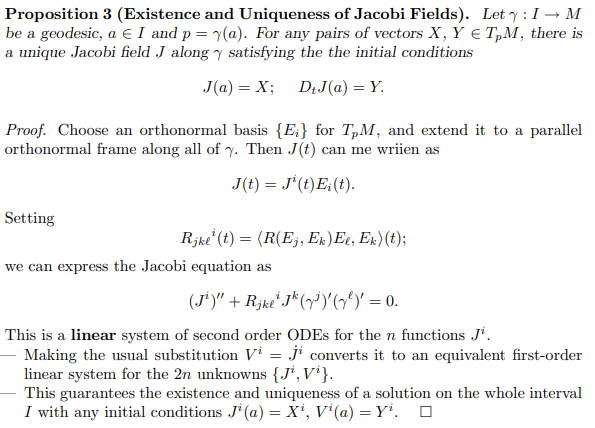
\includegraphics[width = 1\textwidth]{poof}
\end{figure}
{\color{red}{Tehát ha, az I intervallumom a $[-T,T]$ és ebből kiveszek egy tetszőleges pontot, legyen az $-T$, akkor bármilyen 2 kezdőfeltétellel megoldását kapjuk a a Jacobi egyenletnek?}}

\newpage
\section{Dimensionless hamiltonian}

The original hamiltonian:
\begin{equation}
H = -\frac{\hbar^2}{2m} \frac{\partial^2}{\partial x^2} + \underbrace{\frac{\alpha}{2}x^2 + \frac{\beta}{4}x^4}_{\text{double well potential terms}}
\end{equation}
Let $x = \chi x_0$ and substitute it in. Where $\chi$ is now dimensionless.

\begin{equation}
H = -\frac{\hbar^2}{2m} \frac{1}{x_0 ^2} \frac{\partial^2}{\partial x^2} + \frac{\alpha}{2}x_0 ^2 \chi^2 + \frac{\beta}{4}x_0^4 \chi^4
\end{equation}

We only want to keep the coefficients of the interaction and the $x^2$ terms. To do this take the 1st and 3rd terms from the Hamiltonian:
\begin{equation}\label{eq1}
(1) = (3) \rightarrow \frac{\hbar^2}{m x_0 ^2} = \beta x_0 ^4 
\end{equation}
for $x_0$:
$$
x_0 ^6 = \frac{\hbar^2}{m \beta}
$$
\begin{equation}
x_0 = \left( \frac{\hbar^2}{m \beta} \right)^{1/6} = l_d
\end{equation}
For my own peace of mind:
\[
[x_0] = \left( \frac{J^2 s^2}{kg \frac{J}{m^4}} \right)^{1/6} = \left( \frac{J s^2 m^4}{kg} \right)^{1/6}  = \left( \frac{kg \frac{m^2}{s^2} s^2 m^4}{kg} \right)^{1/6} = (m^6)^{1/6} = m \checkmark
\] 

Using this $x_0$ we can tell the energy we measure with:

\begin{equation}
E_0 = \frac{\hbar^2}{m x_0^2} = \left(\frac{\hbar^4 \beta}{m^2}\right)^{1/3} = \beta l_d^4
\end{equation}


\[
[E_0] = \frac{J^2 s^2}{kg m^2} = \frac{J^2}{J} = J \checkmark
\]
Let's turn now to the action integral (without the interaction):
\[
S = \int d\tau L \Rightarrow e^{-\frac{S}{\hbar}}
\]

\begin{equation}
\frac{S}{\hbar} = \int\limits_{-\infty}^\infty d\tau \left\lbrace \frac{m}{2} \dot{x}^2 + \frac{\alpha}{2} x^2 + \frac{\beta}{4} x^4   \right\rbrace
\end{equation}

Here we can make the imaginary time variable dimensionless as well, with the following substitution:

\[
\tau = \tilde{\tau} \tau_0
\]

If we now consider the "$\beta $" term, we can choose $x_0$ and $\tau_0$ in a way that:

\begin{equation}\label{eq7}
1 = \frac{1}{\hbar} \tau_0 \beta x_0^4
\end{equation}

from eq(\ref{eq1}) we can also state this forthe kinetic term:
\begin{equation}\label{eq8}
1 = \frac{1}{\hbar} \frac{x_0^2}{\tau_0} m 
\end{equation} 

By multiplying eq.(\ref{eq7}) and eq.(\ref{eq8}) together we can get rid of $\tau_0$ 
\[
\frac{1}{\hbar^2} x_0^6 \beta m = \frac{1}{\hbar^2} \left( \left( \frac{\hbar^2}{m \beta} \right)^{1/6} \right)^6 \beta m = 1
\]

To calculate $\tau_0$ we can consider eq.(\ref{eq7}) over eq.(\ref{eq8})$^2$:
\begin{equation}
\frac{\frac{1}{\hbar} \tau_0 \beta x_0^4}{\left(\frac{1}{\hbar} \frac{x_0^2}{\tau_0} m \right) ^2} = \frac{\hbar \tau_0^3 \beta}{m^3} = 1
\end{equation}
From this 
\begin{equation}
\tau_0 = \left( \frac{m^2}{\hbar \beta} \right)^{1/3}
\end{equation}

Dimension check:
\[
[\tau_0] = \left( \frac{kg^2}{J s J/m^4} \right)^{1/3} = \left( \frac{kg^2}{kg \frac{m^2}{s^2} s kg \frac{m^2}{s^2}\frac{1}{m^4}}\right)^{1/3} = s \checkmark
\]
Using this $\tau_0$ we can express $E_0$ in another way:
\begin{equation}
E_0 = \frac{\hbar}{\tau_0}
\end{equation}

\subsection{Action integral with the interaction}
Lets write down now the action integral with the interaction:
\begin{equation}
\frac{S}{\hbar} = \int\limits_{-\infty}^\infty d\tilde{\tau} \left\lbrace\frac{1}{2} \left(\frac{\partial \chi}{\partial \tilde{\tau}}\right)^2 + \frac{1}{2} \tilde{\alpha} \chi^2 + \frac{1}{4} \chi^4 + \frac{1}{2} \mu \sum\limits_{i \neq j} \frac{1}{|\chi_i - \chi_j|}\right\rbrace
\end{equation}

Here $\chi \in \left\lbrace\chi_1, \chi_2, ...\right\rbrace$
The emerging $\tilde{\alpha}$ parameter expressed by the previous ones
\begin{equation}
\tilde{\alpha} = \alpha \tau_0 x_0^2 \hbar^{-1}
\end{equation}
Dimension check:
\[
[\tilde{\alpha}] = \frac{J}{m^2} s m^2 \frac{1}{J s} = 1 \checkmark
\]
In this context $\mu$ can be written as:
\begin{equation}
\mu = e^2 k (x_0 \hbar)^{-1} \tau_0
\end{equation}

\subsection{Tunneling distance}
If we now consider the one particle case and make a variable change: $\tilde{\chi} = \frac{\chi}{\chi_0}$ and at the same time lets choose $\chi_0$ as $(-\tilde{\alpha})^{1/2}$

This way the potential term can be written in the following form:
\begin{equation}
V = \chi_0 ^4 \left( \frac{1}{4} \tilde{\chi}^4 - \frac{1}{2} \tilde{\chi}^2\right)
\end{equation}

By taking $\tilde{\tau} = \frac{1}{\chi_0}y $ the action integral takes the form:
\begin{equation}\label{eq16}
\frac{S}{\hbar} = \underbrace{\chi_0^3}_{S_0} \int\limits_{-\infty}^\infty dy \left\lbrace \frac{1}{2} \left( \frac{\partial \tilde{\chi}}{\partial y} \right)^2 + \left( \frac{1}{4} \tilde{\chi}^4 - \frac{1}{2} \tilde{\chi}^2\right) \right\rbrace
\end{equation}

\begin{equation}
S_0 = \left( \frac{-\alpha x_0}{E_0} \right)^{3/2}
\end{equation}

\subsection{Tunneling time scale}
Itt valami nem stimmel!!!
\begin{equation}
\tau_{tun} = \frac{\tau_0}{\chi_0} = \left( \frac{m^2 }{\hbar \beta} \right)^{1/3} \frac{1}{\left(\frac{-\alpha \tau_0 x_0^2}{\hbar}\right)^{1/2}} = \frac{m^{1/3}}{-\alpha^{1/2}}
\end{equation}

\newpage
\section{Scaling}
\subsection{Measurements and constants}
\subsubsection{effective mass}
See fig. S3 in supmat for the measurement: the energy gap present is
\begin{equation}
E_g = 45 \pm 5 \quad meV
\end{equation}
using this measurment on could give an estimate to the electrons effective mass as:
\begin{equation}
v \sim v_{group} \simeq \frac{1}{\hbar} \frac{\partial E}{\partial k}
\end{equation}
 and from 
 \begin{equation}
p = \hbar k 
 \end{equation}
 
 \begin{equation}
 m^\star = \simeq \frac{\hbar k}{v_{fermi}}
 \end{equation}
 
 In our case the effective mass can be calculated as
 \begin{equation}
 m^\star = \frac{E_g}{2 v_f^2}
 \end{equation}
 
 the Fermi velocity in graphene according to \textit{Fermi velocity engineering in graphene by substrate midifcation} ranges from $0.7 \cdot 10^6 \frac{m}{s}$ to $3\cdot 10^6 \frac{m}{s}$.
 
 \begin{align}
 v_f &= a\cdot 10^6 \qquad a\in (0.7, 3) \qquad \frac{m}{s} \\
 1 eV &= 1.602176\dots 10^{-19} \qquad J \\
 m_{e} &= 9.109383 \dots 10^{-31} \qquad kg\\
 \end{align}
 
 using $a=0.8$ we can obtain that the electrons effective mass is 0.0062 times its resting mass.
 
 \begin{equation}
 m^\star = 0.0062 m_e
 \end{equation}
 
 with other $a$ values the multiplirer changes from 0.007 to 0.001.
 
 \subsubsection{Bohr radius}
 
 the Bohr radius can be calculated as
 \begin{equation}
 a_B = \frac{\varepsilon \hbar^2}{e^2 m^\star}
 \end{equation}

 
 \begin{align}
 \hbar &= 1.055\cdot 10^{-34}  &&Js\\
 \varepsilon &= 1 \qquad &&\frac{C^2 s^2}{kg m^3}\\
 e &= -1.60218 \cdot 10^{-19} \qquad &&C\\
 m^\star &= 0.0062 \cdot 9.109838 \cdot 10^{-31} \qquad &&kg
 \end{align}
 
 \begin{align}
 a_B &= \frac{4 \pi \varepsilon \hbar^2}{e^2 m^\star}\\
 &= \frac{4\cdot pi* 8.854\dots 10^{-12} \cdot \left(1.055\dots 10^{-34}\right)^2}{1.602\dots 10^{-19}\cdot 0.0062\cdot 9.109\dots 10^{-31}}\\
 &= 8.535115539186625\cdot 10^{-9}\\
 a_B &= 8.54 \text{ nm}
  \end{align}

 
\subsection{Potential}
The potential has a quatric form:
\begin{equation}
V(x) = E_{p0} \left(\alpha\frac{1}{2}x^2 + \frac{1}{4}x^4 + \varepsilon x \right)
\end{equation}
From some curve fitting the $E_{p0}$ and $\alpha$ parameters can be obtained as well as the $l_d$ length scale, which was calculated above. 
\begin{align*}
E_{p0} &= 1.752  &&\text{dimensionless scaling factor or is it?} \\
\alpha &= -4.119 &&\text{ now its dimensioneless} \\
l_d &= 160 &&\text{nm}
\end{align*}
knowing these we can calculate the nondimensionalized Hamiltonians energy scale:
\begin{equation}
E_0 = 0.48009 \text{ meV}
\end{equation}
and the dimensionless electron interacton factor previously denoted by $\mu$ in the literature its present with $\eta$.
\begin{equation}
\eta = 18.7461
\end{equation}

The experimental results(black) and the fit with the above parameters.
\begin{figure}[!h]
\centering
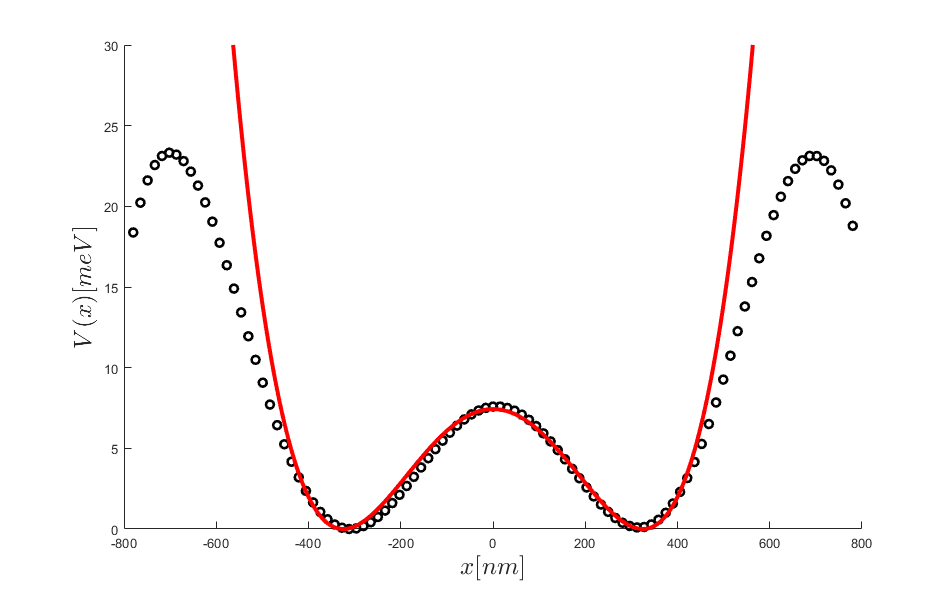
\includegraphics[width=1\textwidth]{final}
\caption{Potential fitting for experimental 4results.m}
\end{figure}



\subsection{Electron interaction parameters.}

A coulomb gas behaviour apart from the temperature depends on the dimensionless ration of the coulomb interaction and the electrons kinetic energy. 

The kinetic part:
\begin{equation}
\left\langle T  \right\rangle \sim N \frac{\hbar^2}{2m^\star} n_e^{2/D}
\end{equation}

In 1 dimensions the electrons' density scales with $1/a$ where $a$ is the inter-electron spacing


And the Coulomb part is:
\begin{equation}
\left\langle U  \right\rangle \sim \frac{e^2}{\varepsilon} n_e^{1/D} N
\end{equation}

the ration of these then follows as:
\begin{equation}
r_s = \frac{\frac{e^2}{\varepsilon}n^{1/D}}{\frac{\hbar^2}{m^\star}n^{2/D}} = \frac{e^2 m^\star}{\varepsilon \hbar^2} n_e^{-1/D}
\end{equation}

but this is not well definied for electron in a quartic potential, because of the not homogeneus electron distribution. Another way to describe this $r_s$ is by the ratio of the inter-electron spacing and the Bohr radius.
\begin{equation}
a_B = \frac{\varepsilon \hbar^2}{m^\star e^2}
\end{equation}

The confinement potential and the kinetic term in the hamiltonian from section 3 yields a natural length scale of the problem as follows:
\begin{equation}
x_0 = l_d = \left( \frac{\hbar^2}{m^\star \beta}  \right)^{1/6}
\end{equation} 

and a characteristic energy as established above:
\begin{equation}
E_0 = \beta^{1/3} \left( \frac{\hbar^2}{m^\star}  \right)^{2/3}
\end{equation}

The parameter that describes the coulomb interaction in the system is denoted by $\mu$ and  is defined similarly as $r_s$, but with $l_d$ instead of $a$.
\begin{equation}
\mu = \frac{l_d}{a_B} = \frac{m^\star e^2}{\varepsilon \hbar^2} \left( \frac{\hbar^2}{m^\star \alpha}  \right)^{1/6}
\end{equation}

given the values of $l_d$ and $a_B$ this quantity is roughly 20 (18.7461 to be consistent). 



Now for the N dependence of the $r_s$ parameter. The potential have the scaling of
\begin{equation}
\chi = \frac{x_i}{x_0} \sim \frac{a}{l_d} \sim \mu^{1/5}
\end{equation}

this implies a scaling parameter :
\begin{equation}
\tilde{r_s} \approx \frac{a}{a_B} = \frac{l_d}{a_B}\frac{a}{l_d} \sim \mu^{6/5}
\end{equation}

\paragraph{Replicating the supmat results somewhat}
I choose an $\alpha$ parameter, and measured the equilibrium positions in the 
\begin{equation}
V(x) = \frac{1}{4}E_p x^4
\end{equation}
potential. Then calculated the inter electron distances in the $l_d = 160 nm$ case. Then made a fit for that data using the $N$ particle number, $\eta$ dimensionless e$^-$ interaction parameter and an arbitrary constant $c$.

{\color{red}{Ábrát érkezik ide; találtak az eredmények}}


\subsection{Összefoglaló az összes kisérleti paraméterről.}
\newpage
\section{Determinant numerical calculation}

\subsection{classical oscillation Frequencies 3particle}
Considering the potential and the interaction terms in a series expanded form:
\begin{align}
V(\chi) &= -\frac{\alpha}{2}\chi^2 + \frac{1}{4}\chi^4 \\
V^\prime (\chi) &= -\alpha \chi + \chi^3\\
V^{\prime\prime} (\chi) &= -\alpha + 3\chi^2
\end{align}

\begin{align}
U(\chi) &= \frac{1}{2}\eta \sum_{j\neq i} \frac{1}{|\chi_i - \chi_j|} \rightarrow U_{1,2} = \eta \left( \frac{1}{\chi_2 - \chi_1} + \frac{1}{\chi_3 - \chi_2}  \right)\\
U^{x,x}_{1,2} (\chi) &= 2\eta \left(\frac{1}{(\chi_2 - \chi_1 )^3} +\frac{1}{(\chi_3 - \chi_1 )^3} \right) \\
U^{x,y} (\chi) &= -2\eta \frac{1}{(\chi_2 - \chi_1)^3} = U_{2,1}^{y,x}\\
\end{align}

having figured these out, we have to solve the following equation:
\begin{equation}
m\ddot{\vec{x}} = -\underline{\underline{D}} \vec{x}
\end{equation}

Then the spring matrix constists of the taylor series second derivatives of the whole ($V+U$) potential:
\begin{equation}
V_{whole} (\chi) = V_0 + 0 + \frac{1}{2}x_i D_{ij} x_j
\end{equation}

\begin{equation}
D_{ij} = \frac{\partial^2 V(\vec{\chi})}{\partial \chi_i \partial \chi_j}
\end{equation}

lets say that
\begin{equation}
\chi_i = A_i e^{i\omega \chi}
\end{equation}

\begin{align}
\ddot{\chi}_i &= -\frac{D_{ij}}{m} \chi_j\\
\omega^2 A_i &= \frac{D_{ij}}{m} A_j
\end{align}

I calculated these numerically using the scaled equilibrium positions, code name: \textit{freqandmode 3p.m}

\subsection{Classical oscillation frequencies for 1 particle}
Same thing as above but for only 1 particle.

\subsection{3 particle propagator}

Goal (42. equation):
\begin{equation}
B = \sqrt{ \frac{2S_0}{\pi}} \left[ \frac{det^\prime \left(-\partial_\tau^2 + V^{\prime \prime}_0 (s_0 (\tau))   \right)}{det\left(-\partial_\tau^2 + \omega^2_N   \right)}  \right]^{-1/2} \times \left[  \frac{det^\prime \left(-\partial_\tau^2 {\bf{1}} + {\bf{\Omega}}^2 (\tau)   \right)}{det\left(-\partial_\tau^2 {\bf{1}}+ {\bf{\Omega}}^2_0   \right)}   \right]^{-1/2}
\end{equation}

The Monte-Carlo trajectory is good for determining the shape of the instanton, but at the beginning of the slope and at the ends it numerically unstable. 

One way to deal with this is fitting a function for the M-C trajectory, but for the rest of the calculations it's best to get back from the "z" $(z\in [-1,1]$) time parametrization to the "y" $(y \in [-\infty, \infty])$ one. The action calculation diverges at $z=\pm 1$, hence the small deviation $(\epsilon = 10^-6)$ from the boundaries. The fitted function generally:
\begin{equation}
\vec{q}(y) = \vec{a} + \vec{b}\tanh(\vec{r}\, y + \vec{c})
\end{equation}

The precision at the edges from the Monte-Carlo trajectory can be achieved with relatively small "$y$" values in the range of 5 - 10. Unfortunately this is a range where consecutive values differ in the order of $10^{16}$.

Because this can be handled like an analytical expression the first derivative of $\vec{q}(\tau \equiv y)$. This way the numerical imperfections can be avoided by using:
\begin{equation}
{\bf{\dot{q}}}(y) = \frac{\vec{b} \vec{r}}{\cosh^2 (\vec{c} + \vec{r}y)}
\end{equation}

to get the unit vectors pointing to the instanton's direction we can still use the ${\bf{q}}$ trajectory.
\begin{equation}
{\bf{e}}(y) = \frac{{\bf{v}}_0 (y)}{|{\bf{v}}_0 (y)|}
\end{equation}

next up is the $\vec{f}$ vector. 
\begin{equation}
\vec{f} = \frac{\Delta \vec{e} - (\vec{e}\Delta \vec{e}) \vec{e}}{\sqrt{|\Delta \vec{e}|^2 - (\vec{e}\Delta\vec{e})^2}}
\end{equation}
where $\Delta\vec{e}$ gives the difference between two unit "e" vectors. The angle between two consecutive unit vectors :
\begin{equation}
\Delta\varphi = 2 \arcsin\left( \frac{|\Delta\vec{e}|}{2}  \right)
\end{equation}

To get the rotation matrix through the instanton I used the previous "e" vectors:
\begin{equation}
R_1 = {\bf{1}} - (\bf{e} \circ \bf{e} + \bf{f} \circ \bf{f}) + (\bf{e}\cdot\bf{e} + \bf{f}\cdot\bf{f})\cos(\Delta  )
\end{equation}

\begin{equation}
R_2 = ({\bf{f}}\cdot{\bf{e}} - {\bf{f}}\cdot{\bf{e}})\sin(\Delta \varphi)
\end{equation}

\begin{equation}
R = R_1 + R_2
\end{equation}

The next thing we need is the eigenvectors of the instanton trajectory at one of its end points, which is already calculated! the rotating Tau vectors then given by the first orthogonal Tau vectors and the rotation matrix.\\

The curvature is given by the 26. eqution in the article:
\begin{equation}
\frac{d \tau_{i,\alpha} (S)}{dS} = C_\alpha (S) \tau_{i,N}(S)
\end{equation}

The derivative can be written in time paramterization as:
\begin{equation}
\frac{d \tau_{i,\alpha} (S)}{dS}  = \frac{d\tau}{dy} \frac{1}{|\vec{v}|}
\end{equation}

and the $N$ index denotes the tau vector which is pointing at the instanton's direction. We know this.
\begin{equation}
\tau_{i,N} = \frac{\vec{v}}{|v|} = \vec{e}
\end{equation}

\begin{equation}
C_\alpha = \tau^\prime \frac{\vec{e}}{|v|}
\end{equation}

Obviously this diverges near the edges, but we only need this for the omega matrix, where it's multiplied by $|v|^2$, so at the edges it's supressed as $|v_0|$ goes to zero.

The omega squared matrix:
\begin{equation}
{\bf{\Omega}}^2_{\alpha,\beta} = \tau_\alpha {\bf{B}} \tau_\beta^T - 3\dot{S}_0^2 (y) C_\alpha (y) C_\beta (y)
\end{equation}


Here B matrix in the 3 particle case is a 3 by 3 matrix, but after multiplying it with the tauspace vectors $\rightarrow$ 2 by 2 matrix. $\dot{S}(y) \equiv |v_0 (y)|$.


\begin{equation}
\Omega^2_{\alpha, \beta} (y) = \tau_\alpha {\bf{B}} \tau_\beta^T - 3 \tau^\prime_\alpha \tau_N \tau^\prime_\beta \tau_N
\end{equation}

\begin{equation}
{\bf{\dot{\Xi}}} = {\bf{\Omega}^2}(y) - {\bf{\Xi}}^2(y)
\end{equation}

\begin{equation}
{\bf{\Xi}}(-T) = {\bf{\Omega}}_0
\end{equation}

this gives us 4 equations to solve, ex.:
\begin{equation}
\Omega_{1,1}(y) - \Xi_{1,1}^2(y) - \Xi_{1,2}(y)\Xi_{2,1}(y) = \frac{d\Xi_{1,1}(y)}{dy}
\end{equation}














\newpage
\section{Codes}
\subsection{Equlibrium positions in the double well potential - Matlab, Simulated annealing}
Code name: \textit{Eq positions - Simulated annealing.m}\\

To determine the positions I used the potential present in the Scaling section. The energy expression is the following:
\begin{equation}
E = E_0 \cdot \left( \frac{a}{2} pos^2 + \frac{1}{4} pos^4  + c \cdot pos \right)
\end{equation}

here $pos$ correspondes to the spatial coordinate, $a$ to the $\alpha$ parameter and during the annealing the $c$ parameter is slowly decreased to zero. This decides that which well the majority of the particles go.

The interaction part:
\begin{equation}
E = E_{pot} + \frac{1}{2} \mu \frac{1}{\left| pos_i - pos_j  \right|}
\end{equation}

The 1/2 factor is present because of the sum; and the $\mu$ denotes the interaction strength. (this was set in the case of 3 particles to 20)

The temperature starts from 300 and decreased with every step exponentially. During a step a random particle is chosen, then a random new position is determined which is proportional to the temperature. There's a limitation to this step, a particle can't jump over another one.

Initial positions are chosen random.

\subsection{1 particle action integral calculations}
In the one particle case the action integral can be calculated analytically. This code was an attempt to get the result decently accurately.
the code name: \textit{numerical integration }\\

There was an attempt to make the action integral's form in a way that its not divergent on the endpoint $z=\pm 1$ but that resulted in other problems. We sticked with a small cut around these points which is denoted by $eps$. The code tests the integral's value through various $eps$ and $r$ values.

The derivative could be evaulated analytically so the integrals form is the following:
\begin{equation}
I = \frac{r}{1-y^2} \frac{1}{(1 + \cosh(\sqrt{2}\,r\,{\arctanh}(y))^2} + \frac{r}{1-y^2}\left(  \frac{1}{4} \left(  \tanh(\arctanh(y) \, r/ \sqrt{2} \right)^2 -1 \right)^2
\end{equation}

the integration then was carried out by the midpoint and trapezoid rules.




\subsection{1 particle tunneling path - Matlab, Simulated annelaing}

\begin{figure}[H]
\centering
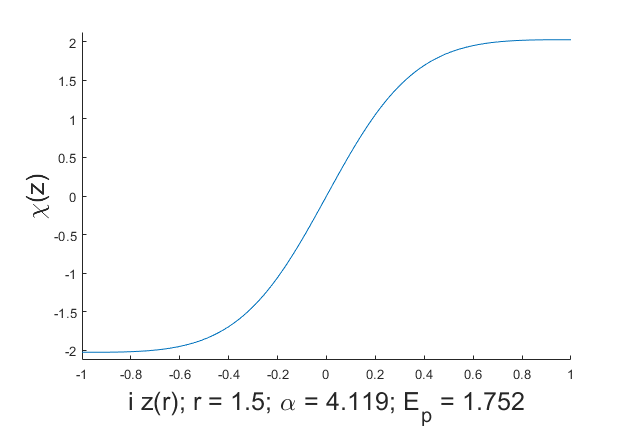
\includegraphics[width = 0.8\textwidth]{1partkhi}
\caption{Experimental parameters used: the Pascu provided data}
\end{figure}

\subsection{3 particle tunneling path - Matlab, Simulated annelaing}


\subsection{•}

\newpage
\section{Proofs}
\subsection{Besel problem}

\subsubsection*{Fourier way}
Let's consider first an arbitrary function $f(x)$. The fourier series of this function is:
\begin{equation}
f(x) = \frac{a_0}{2} + \sum_{n=1}^\infty \left\lbrace a_n \cos\left( \frac{n \pi l}{L}  \right) + b_n \sin \left(  \frac{n \pi l}{L} \right)  \right\rbrace
\end{equation}
where $l\in [l_i,l_f]$ and $L = l_f - l_i$

let $f(x) = x^2$ and $l_i = -l_f = -\pi$ so that $L = 2\pi$

Now the coefficients can be calculated:
\begin{align}
a_0 &= \frac{2}{L} \int_{-\pi}^\pi f(x) dx \\
&= \frac{2}{\pi} \int_0^\pi dx\, x^2\\
&= \frac{2}{3}\pi^2
\end{align}

\begin{align}
a_n &= \frac{2}{L} \int_{-\pi}^\pi dx\, f(x) \cos\left(\frac{n \pi 2 x}{L} \right) \\
&= \frac{2}{\pi }\left.\left(  \frac{x^2 \sin(nx)}{n} \right)\right|_0^\pi - \frac{2}{\pi} \int_0^\pi dx\, \frac{2x \sin(nx)}{n}\\
&=\text{another partial integration later}\\
&= \frac{4 (-1)^n}{n^2}
\end{align}

$b_n = 0$ because $x^2$ is even. So the function now looks like this:
\begin{align}
x^2 &= \frac{2\pi^2}{3\cdot 2} + \sum_{n=1}^\infty \frac{4 (-1)^n}{n^2} \cos\left( \frac{2n\pi x}{L}  \right) \\
&= \frac{\pi^2}{3} + \sum_{n=1}^\infty \frac{4 (-1)^n}{n^2} (-1)^n
\end{align}

now choose $x^2$ tob e equal to 0:
\begin{equation}
\pi^2 = \frac{\pi^2}{3} + \sum_{n=1}^\infty \frac{4}{n^2}
\end{equation}

subtract the $a_0$ term and devide by 4:
\begin{equation}
\frac{\pi^2}{6} = \sum_{n=1}^\infty \frac{1}{n^2}
\end{equation}

\subsubsection*{Complex integral way}

consider the following integral:
\begin{equation}
I = \int_C \frac{1}{z^2} f(z) dz
\end{equation}

let $f(z) $ be the Fermi function:
\begin{equation}
f(z) = \frac{1}{1+ e^{i\pi z}}
\end{equation}

we have several first order poles at $z=\pm (2n + 1 ) =p_n$ and a second order pole at $z=0$.

The residue from the 1st order poles:
\begin{equation}
Res(f(z),p_n) = \lim_{z\rightarrow p_n} (z-p_n) f(z) = \frac{
i}{\pi p_n^2}
\end{equation}

rom the 2nd order pole:
\begin{equation}
Res(f(z),0) = \lim_{z\rightarrow 0} \frac{d}{dz} (z^2 f(z)) = \frac{-\pi i}{4}
\end{equation}

\begin{equation}
\int_C g(z) dz = 2\pi i \sum Res(g(z))
\end{equation}

\begin{equation}
\int_C f(z) dz = 2 \pi i \left(  \frac{
-\pi i}{4} \right) + 2 \pi i \sum_{n=0}^\infty \frac{2i}{\pi (2n+1)^2} = 0
\end{equation}
\begin{align}
\frac{\pi i }{4} &= \sum_{n=0}^\infty \frac{2i}{\pi (2n+1)^2} \\
\frac{\pi^2}{8} &= \sum_{n=0}^\infty \frac{1}{(2n+1)^2}\\
&= \frac{3}{4}\sum_{n=1}^\infty \frac{1}{n^2}
\end{align}

\begin{equation}
\frac{\pi^2}{6} = \sum_{n=1}^\infty \frac{1}{n^2}
\end{equation}
\end{document}